% Chapter 6 is usually termed 'Evaluation' or 'Validation'. How did you test it? In which environment? How
% does it scale? Measurements, tests, screenshots. This chapter will have a volume of 10-15 percent of your
% thesis.
% In this chapter the implementation of Component X is evaluated. An example instance was
% created for every service. The following chapter validates the component implemented in
% the previous chapter against the requirements.
% Put some screenshots in this section! Map the requirements with your proposed solution.
% Compare it with related work. Why is your solution better than a concurrent approach from
% another organization?
% - compare the following approaches:
% suite.st
% http://www.eurofins-digitaltesting.com/test-tools/testwizard-automation-suite/

\chapter{Evaluation\label{cha:chapter6}}

Looking back to chapter \ref{cha:chapter3} describing the requirements of the final product we will
evaluate the result and the usability of it in this chapter. The goal was to create a development
and testing environment for HbbTV applications that is comparable with the state of the art of
modern web development. Building web applications for the big screen turned out to be very cumbersome
since there are no tools that help the developer to understand what is going on on the TV. Common
workarounds are self build logging overlays on the developed application which might give information
about certain variable states but don't disclose the insides of the app at all. The DevTools Backend
component is the first tool that allows HbbTV developer to actually inspect a wide variety of aspects
of an HbbTV application.

\begin{figure}[htb]
  \centering
  \hspace*{-0.7cm}
  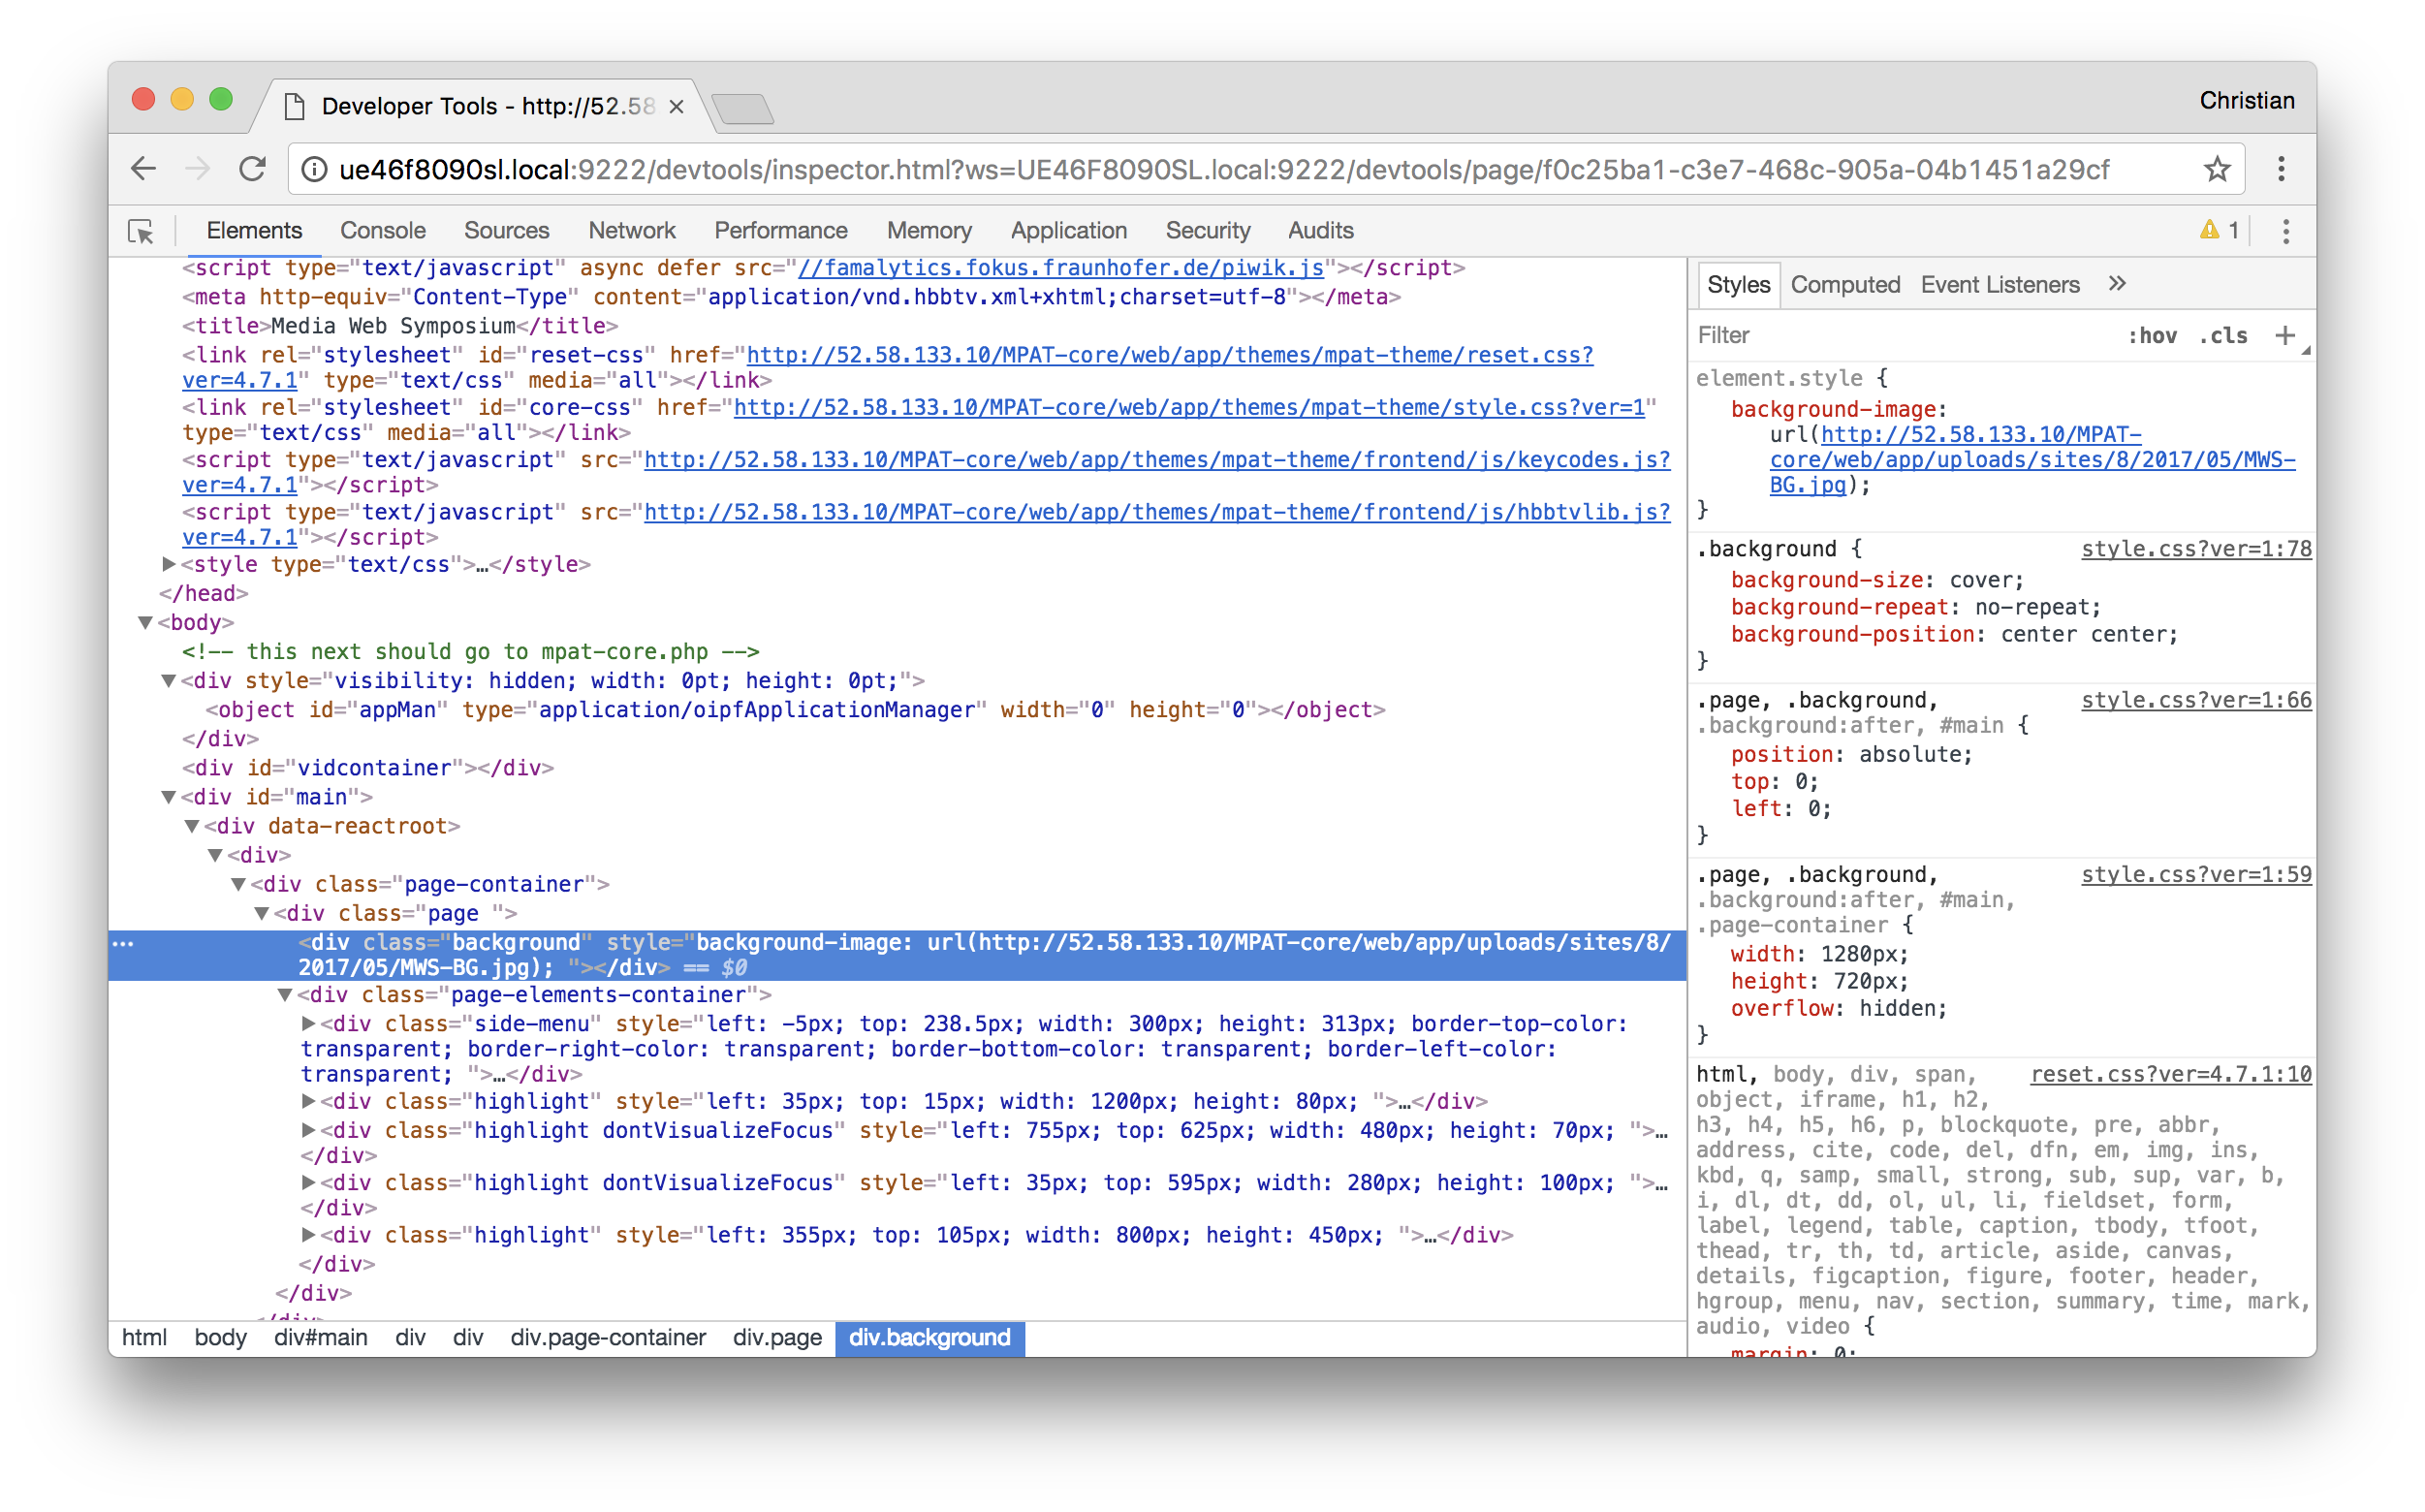
\includegraphics[width=16cm]{elementsPanel.png}\\
  \caption{Debugging the DOM tree of an HbbTV Application using the DevTools application}\label{fig:elementsPanel}
\end{figure}

It not only allows to look into the DOM tree of the app but also modify elements and their CSS
properties. Developer have now the opportunity to build the app directly on the TV instead of
having to implement it on a browser first to then test it on a real Smart TV. Instead building
a custom logging mechanism it automatically captures all logs from the page as well as JavaScript
errors being thrown. In addition to that the \textit{Console} tab of the DevTools application
allows to execute any random JavaScript code within the context of the HbbTV page. With that it
can inspect variables of your application during runtime.

\section{Business model\label{sec:businessmodel}}

- What do they try to solve
- Patent

\section{Features and Offerings\label{sec:features}}

- Explain provided features

\section{Solution Evaluation\label{sec:usab}}

- Compare solutions
- For which group of people is which solution the better choice

\section{Comparison of writing automated tests for web/mobile vs TV\label{sec:diffInWritingTests}}

- Compare Inpute devices
- JS and environement feature set


- Therefor the tool has to be based on existing standards around automated testing and development
